\chapter{Basics of Sweet.JS}

Sweet.js implements macros for JavaScript, which takes source code written with sweet.js macros and produces the expanded source that can be run in any JavaScript environment. 
\section{Type of macros}
\begin{enumerate}
\item {\bf Rule macros }
Rule macros work by matching a syntax pattern and generating new syntax based on the template.
To define rule base macro
\begin{lstlisting}
macro <name> {
  rule { <pattern> } => { <template> }
}
\end{lstlisting} 

Lets write the macro that define swapping of two number
\begin{lstlisting}
	macro swap {
    	rule { ($x, $y) } => {
        	var tmp = $x;
        	$x = $y;
        	$y = tmp;
    	}
	}

	var foo = 5;
	var tmp = 6;
	swap(foo, tmp);
\end{lstlisting} 

When the compiler hits "swap", it invokes the macro and runs each rule against the code after it. When a pattern is matched, it returns the code within the rule. You can bind identifiers \& expressions within the matching pattern and use them within the code.

it might expand to 
\begin{lstlisting}
	var foo = 5;
	var tmp = 6;
	var tmp = foo;
	foo = tmp;
	tmp = tmp;
\end{lstlisting} 
The tmp created from the macro collides with my local tmp. This is a serious problem, but macros solve this by implementing hygiene. Basically they track the scope of variables during expansion and rename them to maintain the correct scope. Sweet.js fully implements hygiene so it never generates the code you see above. It would actually generate this
\begin{lstlisting}
	var foo = 5;
	var tmp$1 = 6;
	var tmp$2 = foo;
	foo = tmp$1;
	tmp$1 = tmp$2;
\end{lstlisting} 
It looks a little ugly, but notice how two different "tmp" variables are created. This makes it extremely powerful to create complex macros elegantly.

\item {\bf Case macros }
Case macro are analogous to syntax-case in Scheme,case macro allow macro author to use javascript code to procedurally create and manipulate the syntax.
To define case base macro
\begin{lstlisting}
	macro <name> {
  		case { <pattern> } => { <body> }
	}
\end{lstlisting}
Example
\begin{lstlisting}
	macro rand {
  	  case { _ $x } => {
    	    var r = Math.random();
     	   letstx $r = [makeValue(r)];
      	 return #{ var $x = $r }
   		}
	}

	rand x;
\end{lstlisting}

Expand To

\begin{lstlisting}
	var x$123 = 0.8367501533161177;
\end{lstlisting}
case is run at expand-time and you use \#\{\} to create "templates" that construct code just like the rule in the other macros.

\end{enumerate}

\section{High level design}

JavaScript macro system, sweet.js, include a separate reader that converts a sequence of tokens into a sequence of token trees,analogous to s-expression in scheme,without feedback from the parser.

\begin{figure}[htb]
\centering
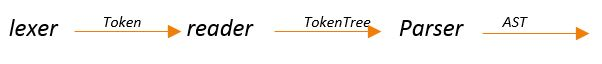
\includegraphics[width=0.5\textwidth]{images/Tokenizer.jpg}
\caption{Sweet.JS anatomy.} 
\label{fig:Tokenizer}
\end{figure}

Here reader records sufficiently history information in the form of token tree in order to decide how to parse the token. 

Example

\begin{lstlisting}
		macro id {
  			case {_ $x } => {
   			 return #{ $x }
  			}
		  }
		id 42
\end{lstlisting}
Reader convert string of token to token tree, 

\begin{figure}[htb]
\centering
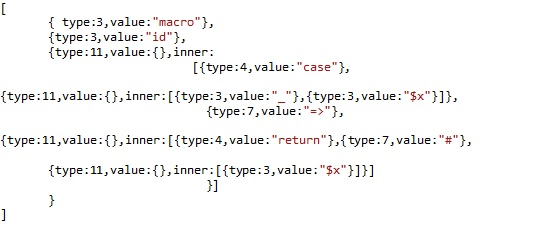
\includegraphics[width=1.0\textwidth]{images/readeroutput.jpg}
\caption{Token tree.} 
\label{fig:readeroutput}
\end{figure}

\begin{figure}[htb]
\centering
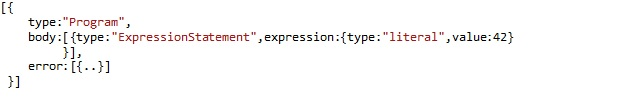
\includegraphics[width=1.0\textwidth]{images/AST.jpg}
\caption{Final AST from parser.} 
\label{fig:AST}
\end{figure}

\section{Problem statement}

Will discuss the issue faced / breaking hygne and anaphoric if